\section{硅和锗的能带结构}

\subsection{硅和锗的导带结构}

根据\fancyref{fml:回旋共振实验}的理论,如果是各向同性材料,则改变磁场方向时只能观察到一个吸收峰,如果是各向异性材料,则改变磁场方向时可能会观察到若干个吸收峰。\goodbreak

而关于硅和锗的实验结果指出,两者属于后一情况,例如对于硅材料来说,实验发现
\begin{itemize}
    \item 若$\vb*{B}$沿$\<1 1 1>$晶轴方向,将观察到一个吸收峰。
    \item 若$\vb*{B}$沿$\<1 1 0>$晶轴方向,将观察到两个吸收峰。
    \item 若$\vb*{B}$沿$\<1 0 0>$晶轴方向,将观察到两个吸收峰。
    \item 若$\vb*{B}$沿任意取向,将观察到三个吸收峰。
\end{itemize}

而关于以上硅的实验事实,我们提出以下硅的导带模型予以揭示:硅是一种各向异性的半导体材料,硅的导带等能面是椭球面,硅的导带最小值(换言之,椭球的位置)并不在$\vb*{k}$空间的原点,而在$\vb*{k}$空间中$[1 0 0]$方向的某个位置,而依据硅晶体立方对称性,这意味着在以下晶向
\begin{Equation}&[xx]
    [1 0 0]\qquad
    [\bar{1} 0 0]\qquad
    [0 1 0]\qquad
    [0 \bar{1} 0]\qquad
    [0 0 1]\qquad
    [0 0 \bar{1}]
\end{Equation}
或者说,在$\<1 0 0>$晶向族给出的六个的相同的位置上,将必然有相同的能量分布,换言之,硅的导带等能面将会是六个对称分布于$\vb*{k}$空间中$k_x,k_y,k_z$正负半轴的椭球面,同时,我们的模型认为,这些椭球面还是以其所在轴为旋转轴(旋转轴为长轴)的旋转椭球面,如\xref{tab:硅的导带结构}所示。\vspace{0.25cm}

\begin{TableLong}[硅的导带结构]{|c|}
    硅的导带结构\\
    \hlinelig
    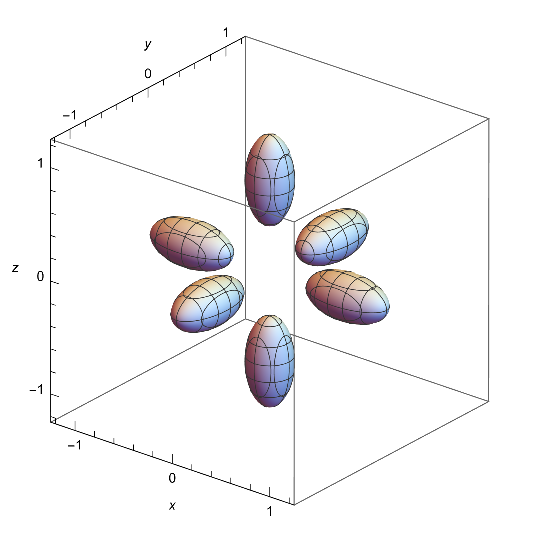
\includegraphics[width=6.5cm]{Mathematica/output/eqE_C.pdf}\\
\end{TableLong}\vspace{0.25cm}
我们很容易列出此时的等能面方程
\begin{Equation}
    E(\vb*{k})=E_c+\frac{\hbar}{2}\qty[
        \frac{(k_x-k_{0x}^s)}{m_{x}^{*s}}+
        \frac{(k_y-k_{0y}^s)}{m_{y}^{*s}}+
        \frac{(k_z-k_{0z}^s)}{m_{z}^{*s}}
    ]
\end{Equation}
其中$s=1,2,3,4,5,6$作为下标分别代表$\<1 0 0>$晶向族的六个晶向,但是,反正这里的六个等能面是完全对称的,我们不妨选取其中一个,例如$[1 0 0]$作为代表晶向进行说明,此时对应的是$k_z$轴正方向上的椭球面,这种情况下,$k_z$是椭球的长轴方向,$k_x,k_y$是椭球的短轴方向。\goodbreak

而为了不失一般性,我们总是将短轴方向的$k$记为$k_1,k_2$,而将长轴方向的$k$记为$k_3$,由于是旋转椭球面,因此,短轴方向有效质量$m_1^{*},m_2^{*}$是相等的,记为$m_t=m_1^{*}=m_2^{*}$,称为\uwave{横向有效质量}(Transverse Effective Mass),长轴方向$m_l=m_3^{*}$,称为\uwave{纵向有效质量}(Longitudinal Effective Mass),这里的横向和纵向可以通过将$k_1,k_2,k_3$置于$k_x,k_y,k_z$来理解。在坐标变换的基础上,还要做两点变化。第一是将坐标原点移至椭球面中心,第二是选取$E_c$为能量零点。

\begin{BoxFormula}[硅的导带等能面]
    硅的导带等能面方程为
    \begin{Equation}
        E(\vb*{k})=\frac{\hbar^2}{2}\qty[\frac{k_1^2+k_2^2}{m_t}+\frac{k_3^2}{m_l}]
    \end{Equation}
    应注意,这仅是一个椭球等能面的方程,而这样的椭球面共有对称分布的六个。
\end{BoxFormula}

而实际上,由于$k_1,k_2$在这里的选取有一个旋转自由度,因此,简单起见,我们不妨指定$k_1$的方向使得磁感强度$\vb*{B}$位于$k_1$和$k_3$轴构成的平面内,并记$\vb*{B}$与$k_3$呈$\theta$角,因此在这个坐标系$k_1,k_2,k_3$中,磁感强度$\vb*{B}$的方向余弦$\alpha,\beta,\gamma$就分别为($\alpha,\beta,\gamma$本身就是方向余弦!)
\begin{Equation}&[1]
    \alpha=\sin\theta\qquad
    \beta=0\qquad
    \gamma=\cos\theta
\end{Equation}

根据\fancyref{fml:回旋共振实验}中$\mne$的表达式
\begin{Equation}&[2]
    \frac{1}{\mne}=\sqrt{\frac{m_1^{*}\alpha^2+m_2^{*}\beta^2+m_3^{*}\gamma^2}{m_1^{*}m_2^{*}m_3^{*}}}
\end{Equation}
这里$m_1^{*}=m_2^{*}=m_t$,而$m_3=m_l$
\begin{Equation}&[3]
    \frac{1}{\mne}=\sqrt{\frac{m_t(\alpha^2+\beta^2)+m_l\gamma^2}{m_t^2m_l}}
\end{Equation}
在\xrefpeq{1}中代入\xrefpeq{3}
\begin{Equation}&[4]
    \frac{1}{\mne}=\sqrt{\frac{m_t\sin^2\theta+m_l\cos^2\theta}{m_t^2m_l}}
\end{Equation}
两端取倒数,提出一个$m_l$,这就得到了硅的导带顶的电子的有效质量的表达式。
\begin{BoxFormula}[硅的导带有效质量]
    硅中的电子,在导带顶部的有效质量为
    \begin{Equation}&[5]
        \mne=m_t\sqrt{\frac{m_l}{m_t\sin^2\theta+m_l\cos^2\theta}}
    \end{Equation}
    其中,$m_t,m_l$分别为横向和纵向有效质量,$\theta$为$\vb*{B}$与$k_3$夹角。
\end{BoxFormula}

现在让我们来验证是否符合硅的实验结果,根据\fancyref{fml:回旋共振实验},每一个有效质量$\mne$就对应一个回旋频率$\omega_c$,因此,晶向族上存在几个有效质量就存在几个回旋频率。

\paragraph{当磁感强度$\vb*{B}$沿晶向族$\<1 1 1>$方向}
其与$6$个晶向$[1 0 0], [\bar{1} 0 0], [0 1 0], [0 \bar{1} 0], [0 0 1], [0 0 \bar{1}]$的夹角均给出$\cos^2\theta=1/3$,故
\begin{Equation}
    \mne=m_t\sqrt{3m_l/(2m_t+m_l)}
\end{Equation}
因此只能观察到一个吸收峰。

\paragraph{当磁感强度$\vb*{B}$沿晶向族$\<1 1 0>$方向}
其与$4$个晶向$[1 0 0], [\bar{1} 0 0], [0 1 0], [0 \bar{1} 0]$的夹角均给出$\cos^2\theta=1/2$,故
\begin{Equation}
    \mne=m_t\sqrt{2m_l/(m_t+m_l)}
\end{Equation}
其与$2$个晶向$[0 0 1], [0 0 \bar{1}]$的夹角均给出$\cos^2\theta=0$,故
\begin{Equation}
    \mne=\sqrt{m_1m_t}
\end{Equation}
因此可以观察到两个吸收峰。

\paragraph{当磁感强度$\vb*{B}$沿晶向族$\<1 0 0>$方向}
其与2个晶向$[1 0 0], [\bar{1} 0 0]$的夹角均给出$\cos^2\theta=1$,故
\begin{Equation}
    \mne=m_t
\end{Equation}
其与$4$个晶向$[0 1 0], [0 \bar{1} 0], [0 0 1], [0 0 \bar{1}]$的夹角均给出$\cos^2\theta=0$,故
\begin{Equation}
    \mne=\sqrt{m_1m_t}
\end{Equation}
因此可以观察到两个吸收峰。

\paragraph{当磁感强度$\vb*{B}$沿任意方向}

而对于$\vb*{B}$的一般方向,将有三种不同的$\cos^2\theta$的值,因而将有三种不同的$\mne$,因此能观察到三个吸收峰,这就圆满的解释了硅的实验结果,说明上述关于硅的导带模型是正确的。

\dotfill\vspace{0.1ex}

硅和锗的导带结构是相似的,但细节上有许多差异。为了明晰这些差异,我们先需要明确一点,硅和锗作为金刚石结构,实质是两个体心立方点阵的套构,因此,硅和锗的形态简约布里渊区与体心立方是一致的,即一个截角八面体(注意,八面体只有六个角),如\xref{fig:金刚石结构的简约布里渊区}所示。\cite{W5}

\begin{Figure}[金刚石结构的简约布里渊区]
    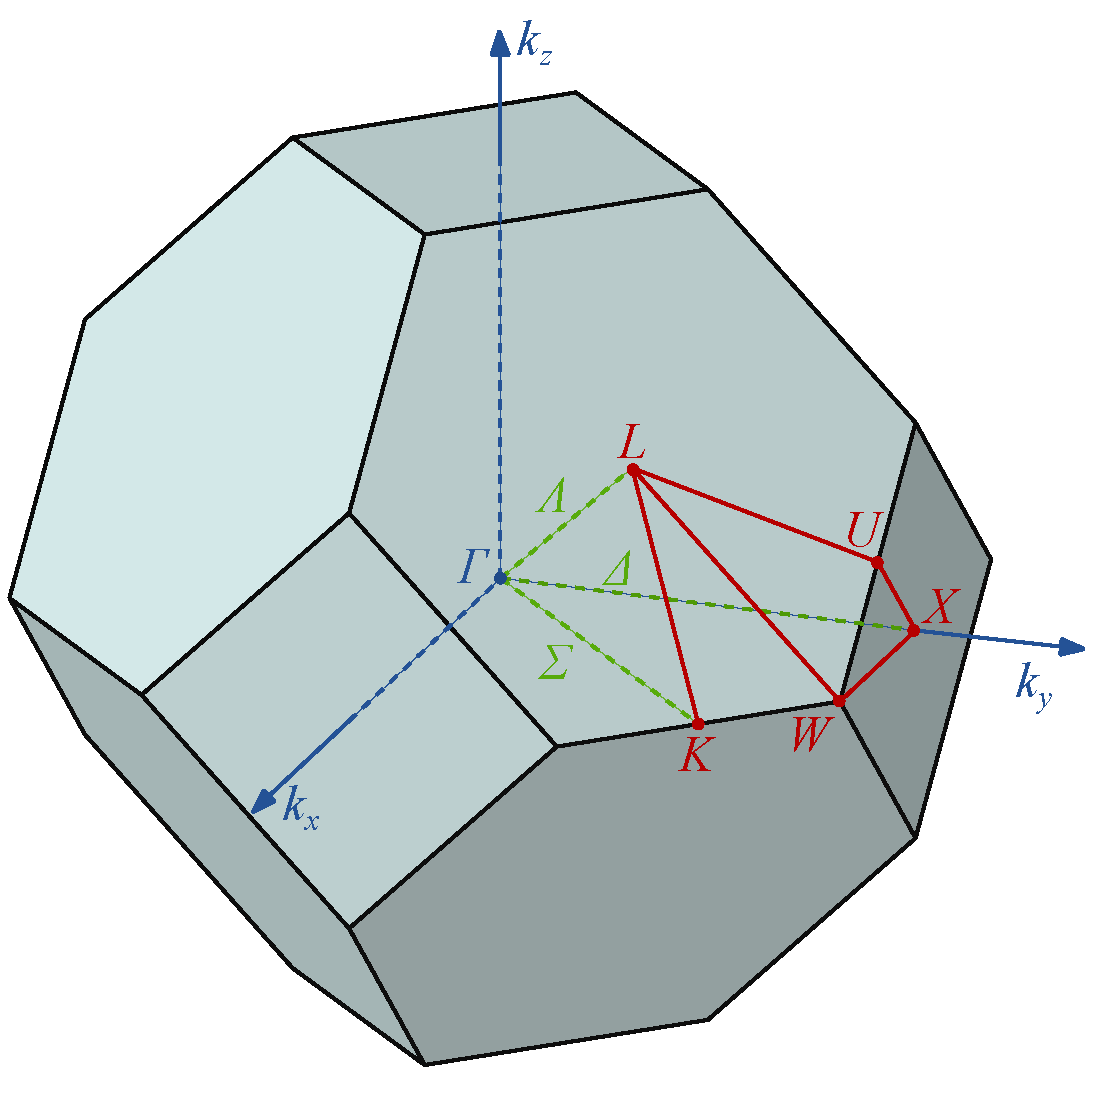
\includegraphics[width=6cm]{image/Brillouin_Zone.pdf}
\end{Figure}

硅和锗的导带等能面均是一系列对称的旋转椭球面,如\xref{fig:硅和锗的导带结构}
\begin{itemize}
    \item 硅共$6$个椭球面,分布在$\<1 0 0>$,即截角八面体的$6$个角的方向,在边界的$0.85$倍处。
    \item 锗共$8$个椭球面,分布在$\<1 1 1>$,即截角八面体的$8$个面的方向,在边界的$1.00$倍处。
\end{itemize}
换言之,锗的$8$个旋转椭球面,其实每个都只有一半落在简约布里渊区内,如\xref{fig:锗的导带结构}所示。
\begin{Figure}[硅和锗的导带结构]
    \begin{FigureSub}[硅的导带结构]
        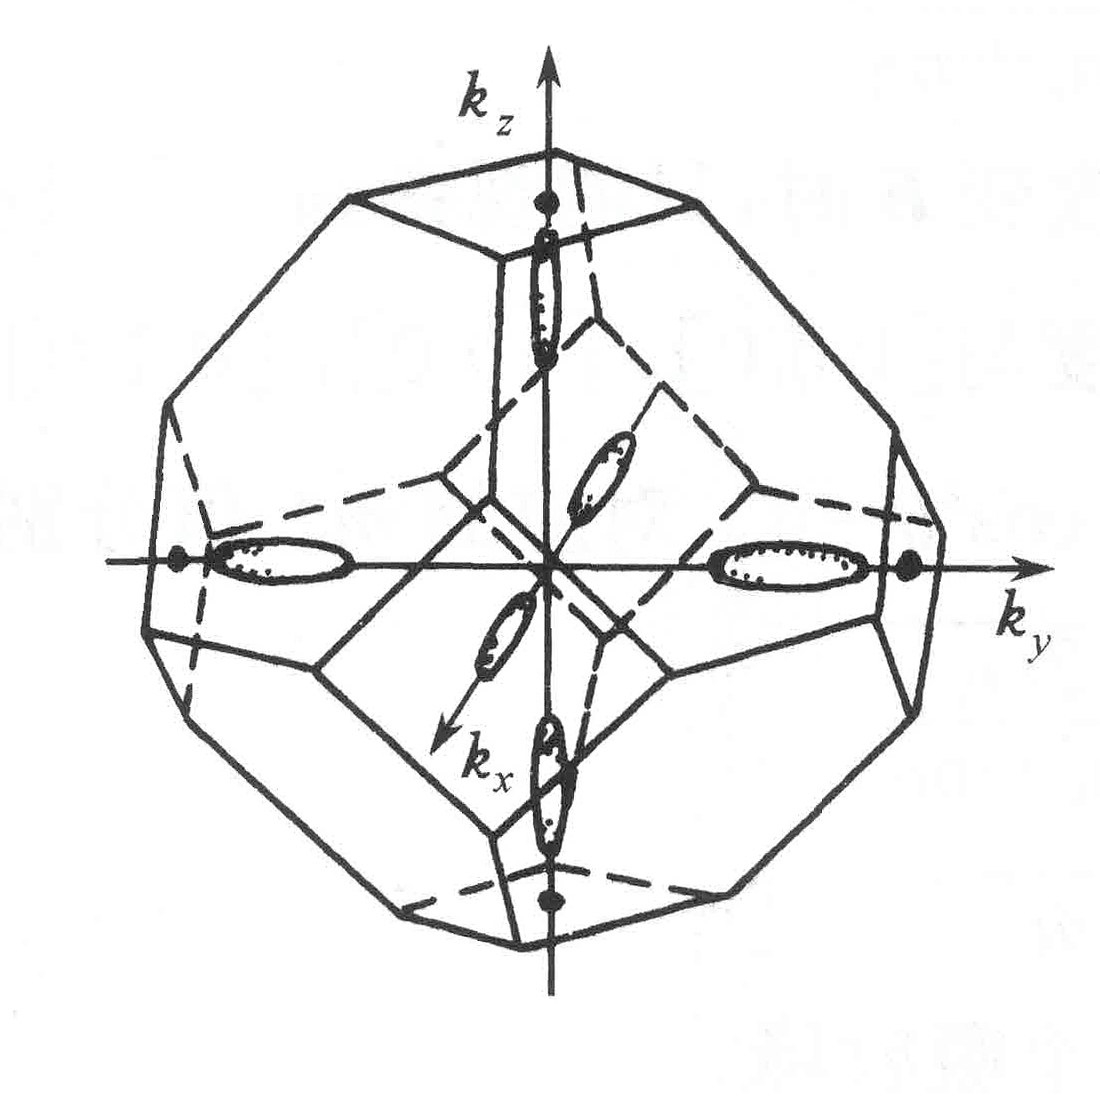
\includegraphics[width=6cm]{image/Si_C.JPG}
    \end{FigureSub}
    \hspace{0.5cm}
    \begin{FigureSub}[锗的导带结构]
        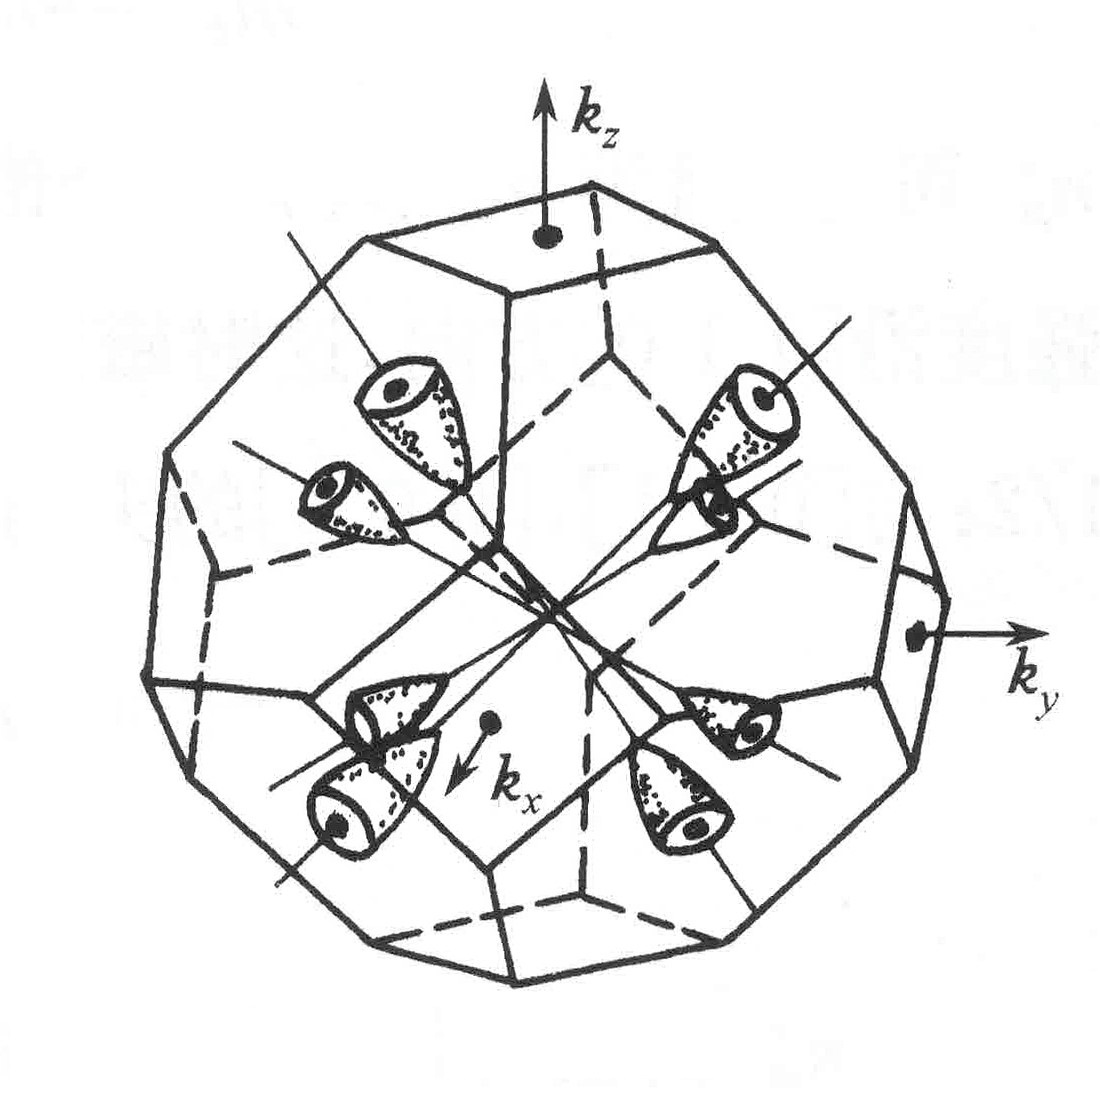
\includegraphics[width=6cm]{image/Ge_C.JPG}
    \end{FigureSub}
\end{Figure}
实验表明,硅的横向有效质量$m_l$和纵向有效质量$m_t$为
\begin{Equation}
    m_l/m_0=0.98\qquad
    m_t/m_0=0.19
\end{Equation}
实验表明,锗的横向有效治疗$m_l$和纵向有效质量$m_t$为
\begin{Equation}
    m_l/m_0=1.64\qquad
    m_t/m_0=0.08
\end{Equation}
因此,锗的椭球似乎应比硅的椭球更长更细(虽然好像图中未能凸显这个特征)。

\subsection{硅和锗的价带结构}
硅和锗的价带结构也可以通过理论计算找到$E(\vb*{k})$和$\vb*{k}$,由回旋共振实验测定其系数,从而计算出空穴的有效质量,但是,由于计算复杂,不做详细讨论,仅对硅的价带结构做定性介绍。

硅的价带结构和导带结构差异比较大,导带极值位于$\vb*{k}\neq 0$处,价带极值则位于$\vb*{k}=0$,即在布里渊区的中心,因此能带是简并的,如果不考虑自旋,价带是三度简并的,如果计入自旋,价带变为六度简并的,计算指出,如果考虑\uwave{自旋--轨道耦合}(Spin–Orbit Coupling)\cite{W6},则可以取消部分简并,可以将六度简并的状态分为两支,一支是二度简并的,一支是四度简并的。
\begin{BoxFormula}[硅的价带结构]
    硅的价带结构可以分为两支,一支是二度简并的,一支是四度简并的。

    四度简并的能量表示为
    \begin{Equation}
        E(\vb*{k})=-\frac{\hbar^2}{2m_0}
        \qty[
            Ak^2\pm
            \sqrt{B^2k^4+C^2(k_x^2k_y^2+k_y^2k_z^2+k_z^2k_x^2)}
        ]
    \end{Equation}
    二度简并的能量表示为
    \begin{Equation}
        E(\vb*{k})=-\Delta-\frac{\hbar^2}{2m_0}Ak^2
    \end{Equation}
    其中$A,B,C$是需要通过回旋共振实验测得的常数,而$\Delta$是自旋--轨道耦合的分裂能量。
\end{BoxFormula}

四度简并的能量表达式中,我们注意到同一个波矢$\vb*{k}$对应两个$E(\vb*{k})$
\begin{itemize}
    \item 取负号时,其对应有效质量较大的空穴,记为$(m_\text{p})_\text{h}$,称为\uwave{重空穴}(Heavy Hole)。
    \item 取正号时,其对应有效质量较小的空穴,记为$(m_\text{p})_\text{l}$\hspace{0.2em},称为\uwave{轻空穴}(Light Hole)。
\end{itemize}

四度简并的两支$E(\vb*{k})$在$\vb*{k}=0$时均有$E=\vb*{0}$,换言之,两者在极值处重合,如果我们从等能面的观点看,随着$\vb*{k}$减小,两者的等能面都会缩小,并在$\vb*{k}\to\vb*{0}$时均会收缩至原点。

二度简并的情形则要简单很多,它的等能面是一个球面,它给出了第三种空穴,其有效质量通常记为$(m_p)_3$。由于自旋--轨道耦合作用,其能量降低了$\Delta$,从而与前面的轻空穴和重空穴的能带分离,对于硅$\Delta=0.04\si{eV}$,对于锗$\Delta=0.29\si{eV}$,由于这个能带离开价带顶(因为$\Delta$的存在使得其在$\vb*{k}=\vb*{0}$时并不会收缩至原点),因此通常来说,我们只会对前两个能带感兴趣。

\begin{Table}[硅和锗的载流子有效质量]{cccccc}
<
\mrx<c>{3}{半导体材料}&\mc{2}(c){电子}&\mc{3}(c){空穴}\\
&纵向&横向&重&轻&第三\\
&$m_l$&$m_t$&$(m_\text{p})_\text{h}$&$(m_\text{p})_\text{l}$&$(m_\text{p})_3$\\
>
硅&$0.98m_0$&$0.19m_0$&$0.53m_0$&$0.16m_0$&$0.25m_0$\\
锗&$1.64m_0$&$0.08m_0$&$0.28m_0$&$0.04m_0$&$0.07m_0$\\
\end{Table}\nopagebreak
在\xref{tab:硅和锗的载流子有效质量}中,我们整理了硅和锗中的电子和空穴的有效质量。

在\xref{tab:硅的价带结构}中,我们列出了重空穴、轻空穴、第三空穴的等能面,可以看出,第三空穴的等能面就是球面,重空穴的等能面类似立方体(表面有些凹陷),轻空穴的等能面类似正八面体。

\begin{TableLong}[硅的价带结构]{|c|}
    硅的价带结构--重空穴\\*
    \hlinelig 
    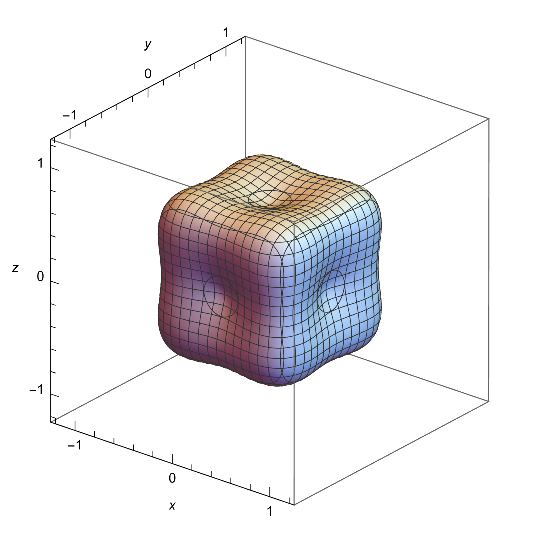
\includegraphics[width=6.5cm]{Mathematica/output/eqE_V1.pdf}\\
    \hlinemid
    硅的价带结构--轻空穴\\*
    \hlinelig
    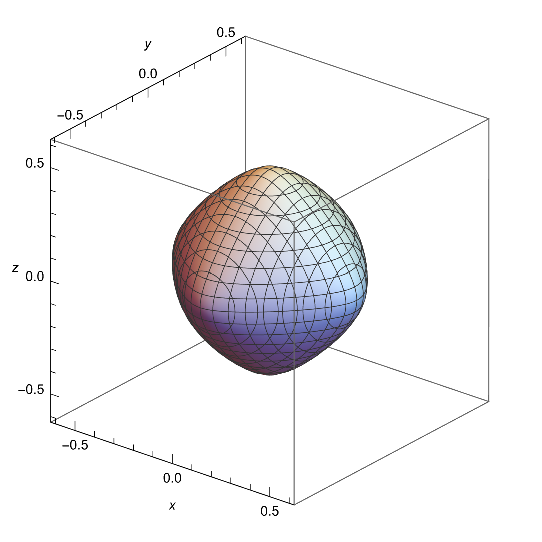
\includegraphics[width=6.5cm]{Mathematica/output/eqE_V2.pdf}\\
    \hlinemid
    硅的价带结构--第三空穴\\*
    \hlinelig
    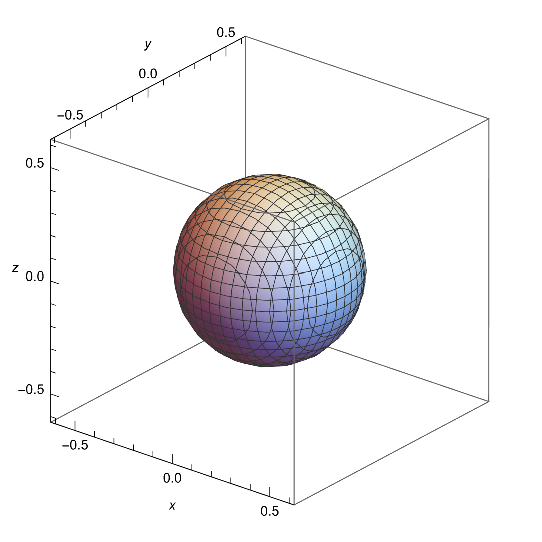
\includegraphics[width=6.5cm]{Mathematica/output/eqE_V3.pdf}\\
\end{TableLong}

\subsection{硅和锗的能带图}
通过以上讨论我们可以看到,硅和锗作为三维中的实际半导体材料,其能带结构是非常复杂的,因此在实践中,我们往往会选取一些对称性比较好的方向来刻画半导体能带的主要特点。
\begin{Figure}[硅和锗的能带图]
    \hspace{0.25em}
    \begin{FigureSub}[硅的能带图]
        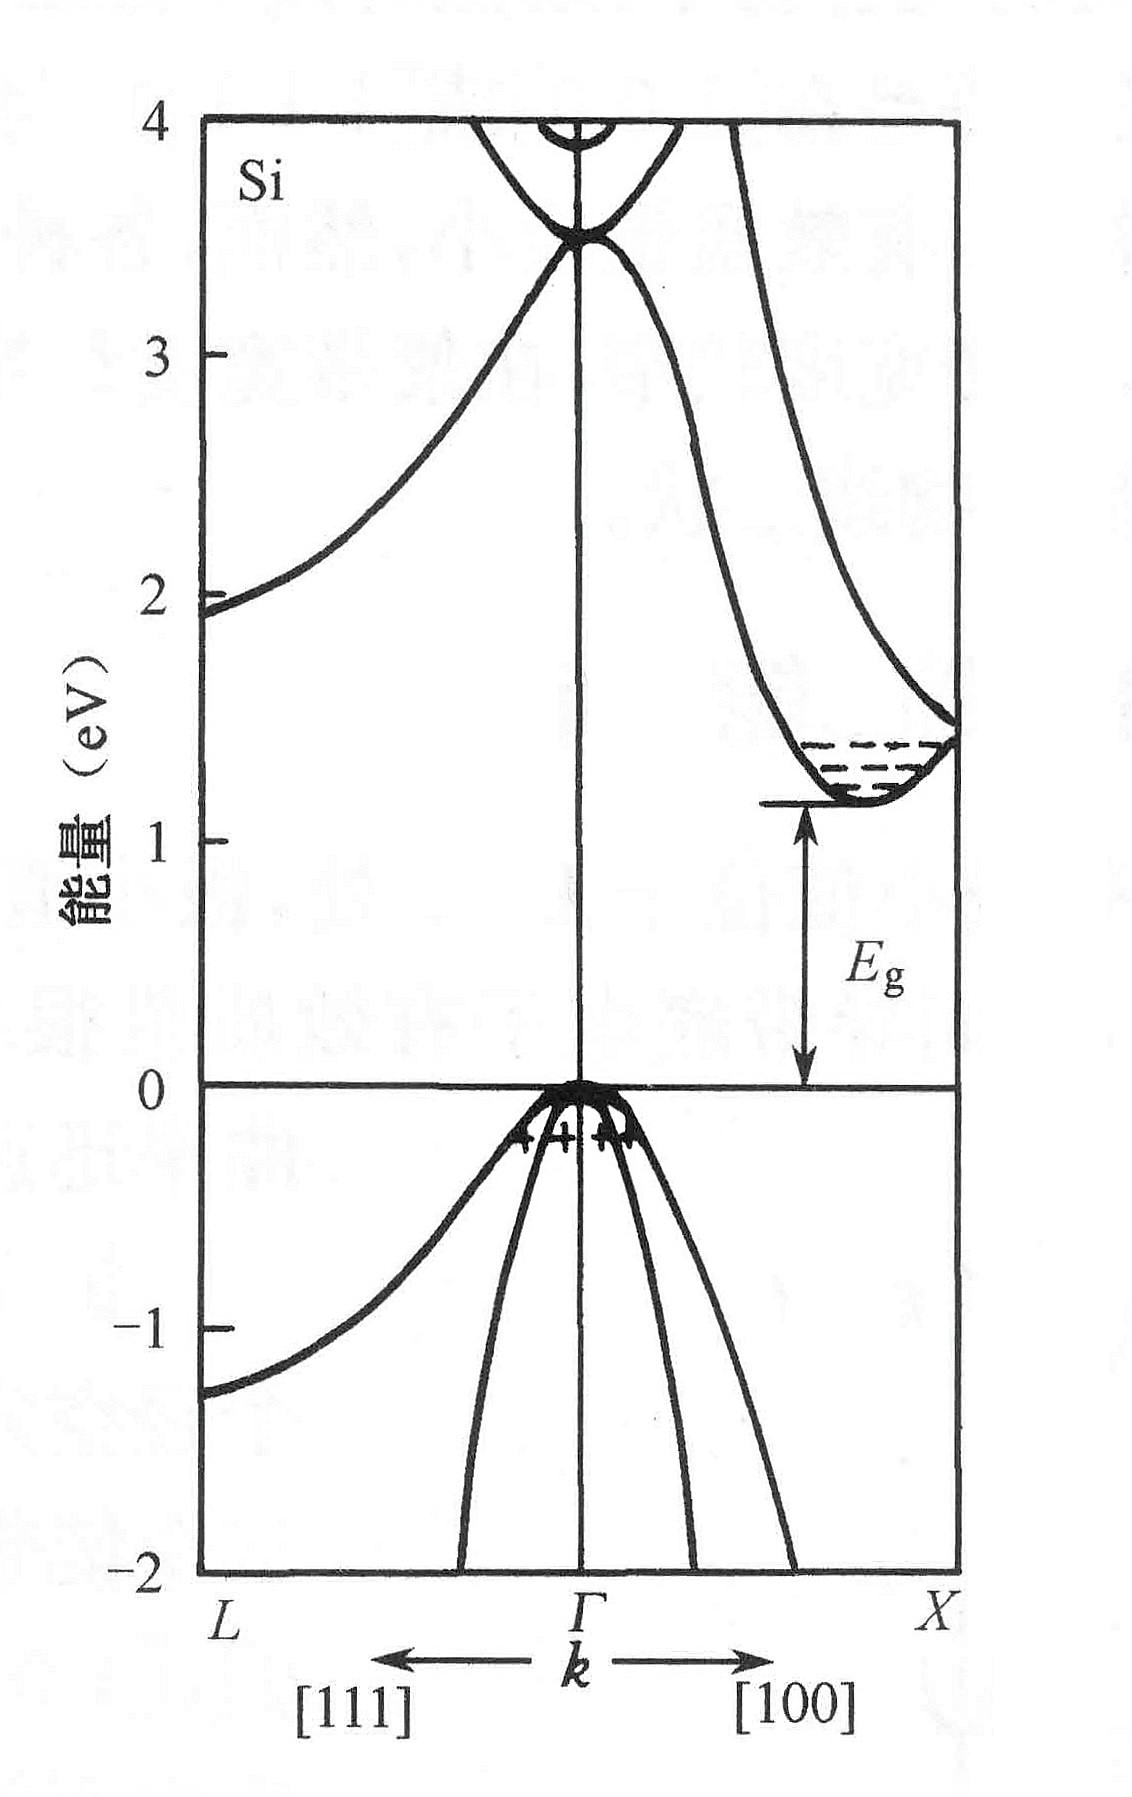
\includegraphics[width=5.37cm]{image/Ge_Band.jpg}
    \end{FigureSub}
    \hspace{1.5em}
    \begin{FigureSub}[锗的能带图]
        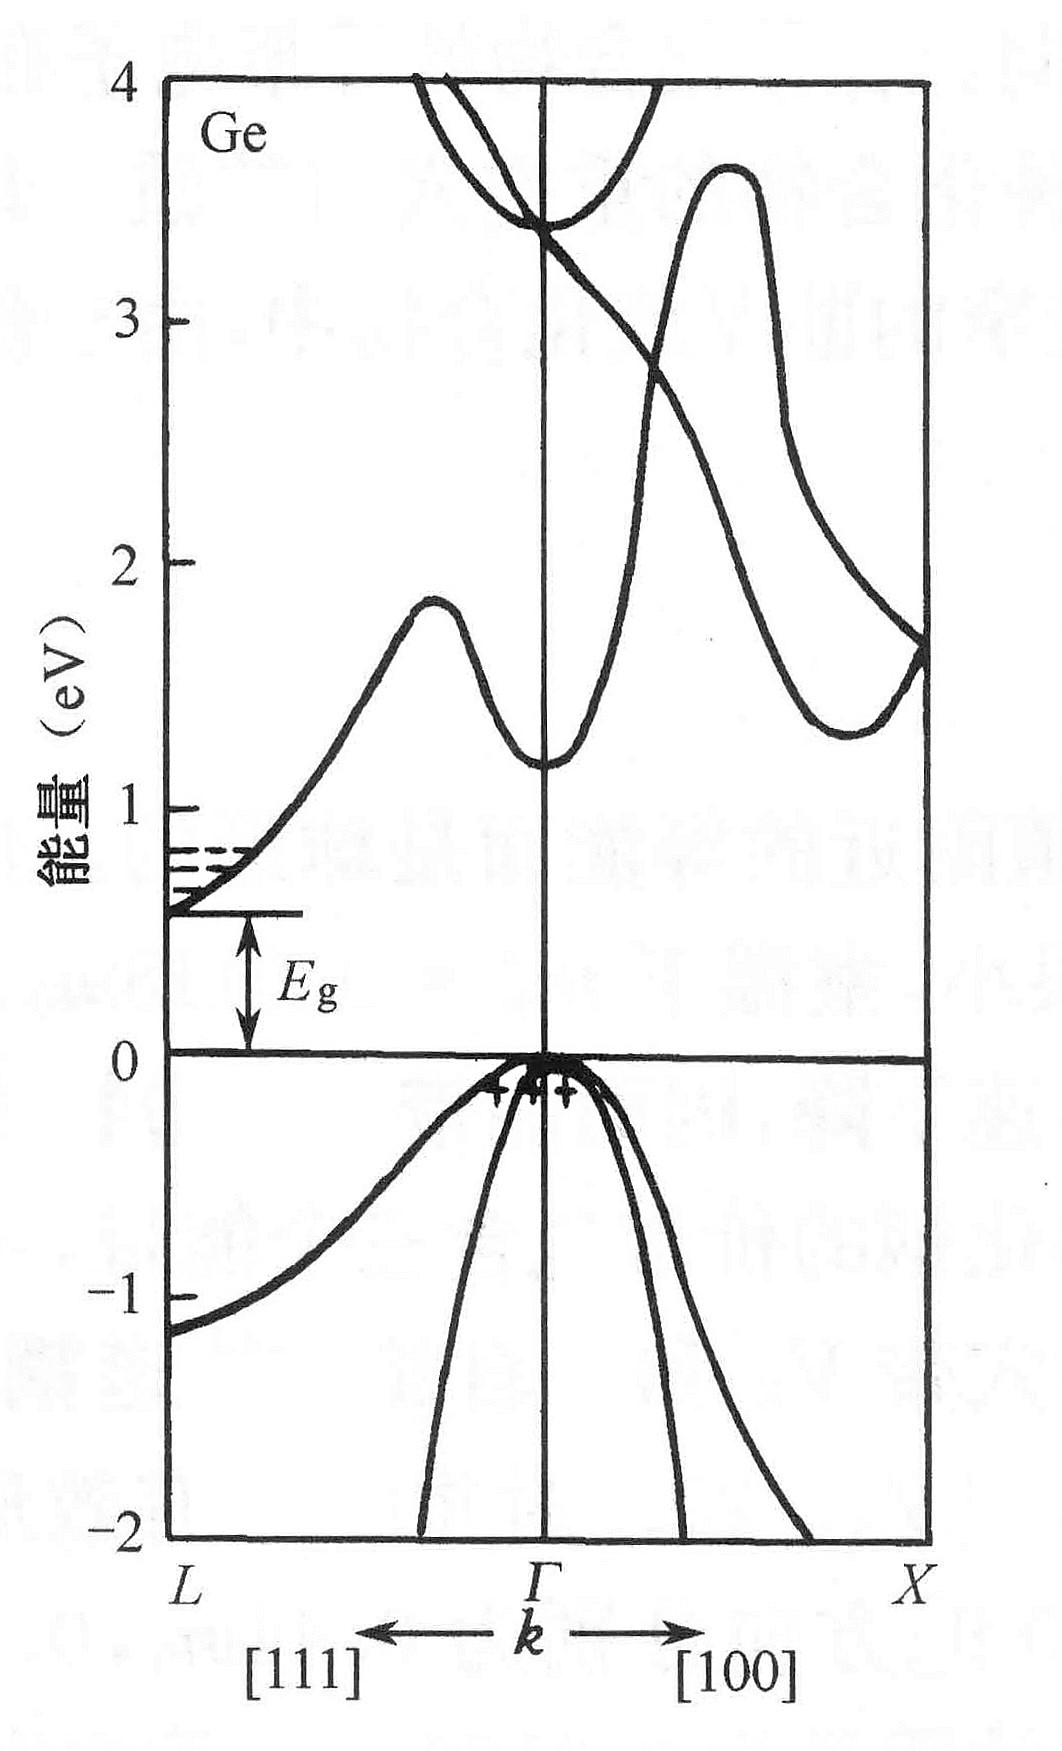
\includegraphics[width=5cm]{image/Si_Band.jpg}
        \vspace{0.1cm}
    \end{FigureSub}
\end{Figure}

虽然能带图看起来很复杂,但是其实是可以部分理解的
\begin{itemize}
    \item 能带图的左右两部分,是两个晶向上的$E(k)$曲线,如\xref{fig:金刚石结构的简约布里渊区}所示,符号$\Gamma$代表原点
    \begin{itemize}
        \item 符号$X$代表$\<1 0 0>$晶向上与简约布里渊区六个角的交点,故右端为$\<1 0 0>$晶向。
        \item 符号$L$\hspace{0.55em}代表$\<1 1 1>$晶向上与简约布里渊区八个面的交点,故左端为$\<1 1 1>$晶向。
    \end{itemize}
    \item 能带图中,上半部分为导带曲线,下半部分为价带曲线,\xref{subsec:硅和锗的价带结构}中曾提到过,价带有三支,这里只绘制了重空穴和轻空穴对应的曲线,两者的价带顶确实在原点处重合。
\end{itemize}
这里我们注意到,硅和锗的能带中,价带顶和导带底所对应的$\vb*{k}$是不同的,我们将这种带隙称为\uwave{间接带隙}(Indirect Band Gaps),而过去那种理想的,价带顶和导带底所对应的$\vb*{k}$是相同的那种情况,我们称为\uwave{直接带隙}(Direct Band Gaps)。两者的主要差异在于,直接带隙在能带跃迁时只会释放或吸收光子,间接带隙在此基础上,由于$\vb*{k}$导致的动量改变,还需要额外释放或吸收声子,故光电器件通常会使用直接带隙的半导体材料制造,而不会使用硅和锗。

这里还要指出的是,禁带宽度$E_\text{g}$其实是会随着温度升高而减小的。直观上很容易理解,随着温度的升高,电子的热运动加剧,变得更活跃,因此从价带跃迁至导带就变得更为容易了。
\begin{BoxFormula}[禁带宽度和温度的关系]
    禁带宽度和温度的关系如下
    \begin{Equation}
        E_\text{g}(T)=E_\text{g}(0)-\frac{\alpha T^2}{T+\beta}
    \end{Equation}
    其中,$\alpha$和$\beta$是关于材料的温度系数。
\end{BoxFormula}

在\xref{tab:硅和锗的禁带性质}中,我们整理了硅和锗与禁带有关的性质
\begin{Table}[硅和锗的禁带性质]{cccc}
    <
    \mrx<c>{2}{半导体材料}&禁带宽度(绝对零度)&\mc{2}(c){\hspace{3em}温度系数}\\
    &$E_\text{g}(0)$&$\alpha$&$\beta$\\
    >
    硅&$1.170\si{eV}$&$4.73\times 10^{-4}\si{eV. V^{-1}}$&$636\si{K}$\\
    锗&$0.744\si{eV}$&$4.78\times 10^{-4}\si{eV. V^{-1}}$&$235\si{K}$\\
\end{Table}
这里可以看出,硅的禁带宽度实际上是大于锗的禁带宽度的。